\documentclass{article} 
\usepackage{tikz} 
\begin{document} 
	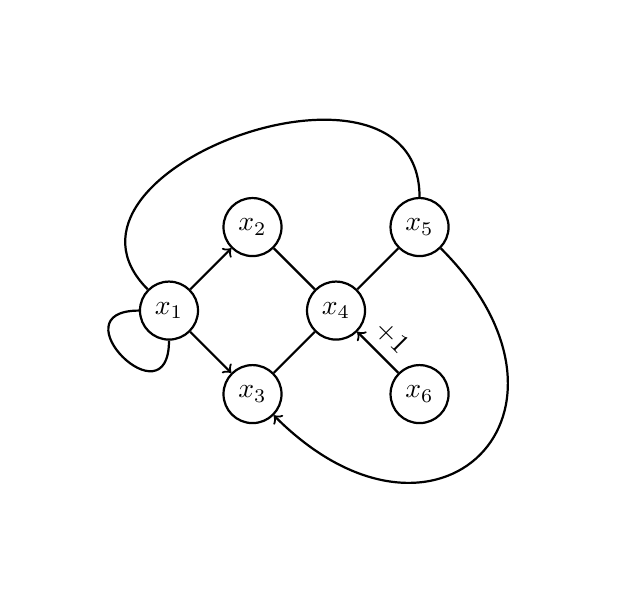
\begin{tikzpicture}[node distance={15mm}, thick, main/.style = {draw, circle}] 
		\node[main] (1) {$x_1$}; 
		\node[main] (2) [above right of=1] {$x_2$}; 
		\node[main] (3) [below right of=1] {$x_3$}; 
		\node[main] (4) [above right of=3] {$x_4$}; 
		\node[main] (5) [above right of=4] {$x_5$}; 
		\node[main] (6) [below right of=4] {$x_6$}; 
		\draw[->] (1) -- (2); 
		\draw[->] (1) -- (3); 
		\draw (1) to [out=135,in=90,looseness=1.5] (5); 
		\draw (1) to [out=180,in=270,looseness=5] (1); 
		\draw (2) -- (4); 
		\draw (3) -- (4); 
		\draw (5) -- (4); 
		\draw[->] (5) to [out=315, in=315, looseness=2.5] (3); 
		\draw[->] (6) -- node[midway, above right, sloped, pos=1] {+1} (4); 
	\end{tikzpicture} 
\end{document}